\documentclass[12pt,oneside]{book}
% pouzite balicky
\usepackage[utf8]{inputenc}
\usepackage{amsmath}
%\usepackage[]{babel}

\RequirePackage{ifpdf}
\ifpdf
  \RequirePackage[pdftex]{graphicx}
  \RequirePackage[pdftex]{color}
  \RequirePackage{ps4pdf}
\else
  \RequirePackage[dvips]{graphicx}
  \RequirePackage[dvips]{color}
  \RequirePackage{pstricks}
\fi

\usepackage{pst-all}

\usepackage{pslatex}
\usepackage{url}
%% Define a new 'leo' style for the package that will use a smaller font.
\makeatletter
\def\url@leostyle{%
  \@ifundefined{selectfont}{\def\UrlFont{\sf}}{\def\UrlFont{\small\ttfamily}}}
\makeatother
%% Now actually use the newly defined style.
\urlstyle{leo}

%\usepackage{hyperref}
%\usepackage{html}

\usepackage{listings}
\usepackage{array}
\usepackage{multirow}
\usepackage{comment}
\usepackage{lscape}
\usepackage{rotating}
\usepackage{amssymb}

%\usepackage{nopageno}
\usepackage{geometry}
\geometry{paperwidth=8.26in,paperheight=11.69in,
          left=4cm,right=3cm,
          top=3.5cm,bottom=3.5cm}

\usepackage{float}
\floatstyle{ruled}

\newfloat{algorithm}{thp}{loa}
\floatname{algorithm}{Algoritmus}

\newtheorem{definition}{Definice}

\newcommand{\etalchar}[1]{$^{#1}$}
\sloppy
%%%%%%%%%%%%%%%%%%%%%%%%%%%%%%%%%%%%%%%%%%%%%%%%
\title{Implementace algoritmů pro zpracování obrazu na IBM Cell}
\author{Václav Klecanda}
\date{29.4.2009}
\begin{document}

\pagestyle{empty}

\begin{center}


\large
\textsc{
Univerzita Karlova v~Praze\\
Matematicko-fyzikální fakulta\\[1.2cm]
}

%%%%%%%%%%%%%%%%%%%%%%%%%%%%%%%%%%%%%%%%%%%%%%%%%%%%%%%%%%%%%%%%%%%%%%%%%%%%%%%%
%   diplomova prace

\Huge
\textbf{
DIPLOMOVÁ PRÁCE\\[1.5cm]
}

%%%%%%%%%%%%%%%%%%%%%%%%%%%%%%%%%%%%%%%%%%%%%%%%%%%%%%%%%%%%%%%%%%%%%%%%%%%%%%%%
%   logo skoly


\includegraphics[height=7.5cm]{data/logo.eps}\\[2cm]

%%%%%%%%%%%%%%%%%%%%%%%%%%%%%%%%%%%%%%%%%%%%%%%%%%%%%%%%%%%%%%%%%%%%%%%%%%%%%%%%
%   vypracoval

\Large
Václav Klecanda\\[1cm]

%%%%%%%%%%%%%%%%%%%%%%%%%%%%%%%%%%%%%%%%%%%%%%%%%%%%%%%%%%%%%%%%%%%%%%%%%%%%%%%%
%   titulek
\LARGE
\textbf{
Implementace na Cell\\[1cm]
}

%datum
\normalsize
Duben 2007\\[1.5cm]

%%%%%%%%%%%%%%%%%%%%%%%%%%%%%%%%%%%%%%%%%%%%%%%%%%%%%%%%%%%%%%%%%%%%%%%%%%%%%%%%
%   katedra
\large
\textbf{
Kabinet software a výuky informatiky\\
}

%%%%%%%%%%%%%%%%%%%%%%%%%%%%%%%%%%%%%%%%%%%%%%%%%%%%%%%%%%%%%%%%%%%%%%%%%%%%%%%%
%   vedouci
Vedoucí diplomové práce: \textbf{Mgr. Václav Krajíček}\\

%%%%%%%%%%%%%%%%%%%%%%%%%%%%%%%%%%%%%%%%%%%%%%%%%%%%%%%%%%%%%%%%%%%%%%%%%%%%%%%%
%   program
Studijní program: \textbf{Informatika}

\end{center}

\pagebreak
 

\pagestyle{empty}


\vspace*{1em}




%%%%%%%%%%%%%%%%%%%%%%%%%%%%%%%%%%%%%%%%%%%%%%%%%%%%%%%%%%%%%%%%%%%%%%%%%%%%%%%%
%   Pod�kov�n�

\begin{figure}[t]

\par
%D�kuji RNDr. Pelik�novi za cenn� rady a p�ipom�nky k~t�to pr�ci. MUDr. Hor�kovi za poskytnut� l�ka�sk�ch znalost� a dat. Mgr. Mar��lkovi za pomoc a podporu.

\end{figure}

%\pagebreak




%%%%%%%%%%%%%%%%%%%%%%%%%%%%%%%%%%%%%%%%%%%%%%%%%%%%%%%%%%%%%%%%%%%%%%%%%%%%%%%%
%   Prohl��en�

\vspace*{1em}

\flushbottom

\begin{figure}[b]

\par
%Prohla�uji, �e jsem svou diplomovou pr�ci napsal(a) samostatn� a v�hradn� s~pou�it�m citovan�ch pramen�. Souhlas�m se zap�j�ov�n�m pr�ce.

\vspace{2em}

\begin{tabular*}{1.0\textwidth}[b]{@{\extracolsep{\fill}} l r }
%V~Praze dne 20. Dubna 2007 & V�clav Kraj��ek\\
                           %& vlastnoru�n� podpis
\end{tabular*}

\vspace*{2em}

\end{figure}

\raggedbottom

%%%%%%%%%%%%%%%%%%%%%%%%%%%%%%%%%%%%%%%%%%%%%%%%%%%%%%%%%%%%%%%%%%%%%%%%%%%%%%%%
%   KONEC Podekov�n�
 

\pagestyle{empty}

\tableofcontents
\pagebreak

\listoffigures
\pagebreak

\listoftables
\pagebreak

%\listof{algorithm}{Seznam algoritmu}

\pagebreak

%--------------------------------------------------------
%-------------           ABSTRAKT           -------------
%--------------------------------------------------------

\section*{submission}
Study available literature and technical documentation about programming on IBM Cell BE architecture. As well as interfaces, development environments and tools for creating programs for CellBE and its particular implementation Play Station 3, IBM system simulator, Cell Blade. Find out its potential and abilities for parallel processing. Learn about design patterns.

Try some algorithm (registration, segmentation) aimed to medical data processing (CT, MR, X-ray images) where huge data sizes are processed and where results has to be get relativelly fast because diagnosis are made for lasg number of patients. It suitable to do comparation study between common PC architecture and CellBE aimed to speed, precision, code complexity and ways of algorithms design itselfs. 

\pagebreak

%vkladani headeru
\pagestyle{headings}

%\setlength{\parindent}{0pt}
\setlength{\parskip}{2ex}

\chapter{CellBE platform}

This chapter will introduce CellBE (Cell Broadband Engine) itself, its specifics. Introduce to my experience with the platform will then follow.

\section{About the processor}

CellBE processor is representative of new generation of IBM's CellBE platform family made by collaboration of IBM, Sony, and Toshiba. CellBE is an asymmetric, high-performance multi-core processor that combines eight synergistic processing elements (SPEs) and a Power Processing Element (PPE), which is a general-purpose IBM Power PC\textregistered core. Each SPE has a 4-way SIMD engine, a high-speed local store and a direct memory access (DMA) engine. The 4-way SIMD unit of each SPE can perform a floating or integer operation on four data elements at every clock tick. Unlike conventional microprocessors, each SPE does not have a hardware cache to manage its small on-chip local store. All the elements are connected through high speed bus (EIB - Element Interconnect Bus). Therefore, this architecture can be viewed as a distributed memory multiprocessor with a very small local memory (local store), under software control, attached to a larger (central) shared memory through DMA engine that manages transfering data from central memory to local store and vice versa.

CellBE achieves a significant performance per Watt and performance per chip area advantage over conventional high-performance processors, and is significantly more flexible and programmable than single-function and other optimized processors such as graphics processors, or conventional digital signal processors. While a conventional microprocessor may deliver about 20+GFlops of single-precision (32b) floating-point performance, Cell delivers 200+ GFlops (in ideal conditions) at comparable power.

A number of signal processing and media applications have been implemented on Cell with excellent results. Advanced visualization such as ray-casting, ray-tracing, and volume rendering. Streaming applications such as media encoders and decoders and streaming encryption and decryption standards have also been demonstrated to perform about an order of magnitude better on Cell than on conventional PC.

TODO obrazek Cellu
\begin{figure}
    \centering
    \includegraphics[height=7.9cm]{medatlas}
    \caption[CellBE processor layout]{Anatomick� atlas - horn� ��st b�icha zep�edu.
      Jsou zde dob�e vid�t ledviny (zelen�).
      Prav� je ��ste�n� p�ekryt� dvan�ctern�kem.
      Slezina (�erven�) le�� vlevo zhruba v~�rovni ledvin a j�tra (mod�e) le�� vpravo vep�edu o~n�co v��e.
      Na obr�zku je vid�t jen jejich ��st.}
    \label{fg:processorLayout}
\end{figure}

\subsection{PPE - PowerPC\textregistered Processing Element}
PPE is derived from IBM Power PC\textregistered core. Has 512kB L2 cache in die. It supports the Power Architecture ISA, inherits the memory translation, protection, and SMP coherence model of mainstream 64-bit Power processors. CBEA also supports virtualization (logical partitioning), large pages, and other recent innovations in the Power architecture. Programming for the PPE is the same as for conventional processors.

\subsection{SPU - Synergistic Processing Element}
SPE is an autonomous processor (sometimes called accellerator) targeted for computational intensive applications. It supports a SIMD-RISC instruction set. Has 128 (128-bit long) unified registers to store all types of data (in contrast from traditional RISCs where registers are devided according data types). One of CellBE programming aspects is converting the code that it uses the SIMD instructions. This process is calleed "SIMDation".

SPE stores its program and data in its associated local storage memory as private memory. DMA transactions are used to tranfer data from/to central memory as well as between two local stores. We say that data is "DMAed" from source to destination. DMA commands can be issued in many ways. Synchronous, asynchronous, in scatter-gaether manner through DMA lists. This memory management is another big part of programming for CellBE.

Programming for SPE has some differencies over programming for conventional processor. You have always to count with the fact you have only 256kB for your program and data. Data is 

This processor is embeded in Sony Playstation 3 game console as well as IBM Blade servers where two or more such processors (as building blocks) connected by high speed bus creates powerfull and modular machine. I have PlayStation3 machine available for my work.

\section{My journey into CellBE platform}
When I started this work I was Windows\textregistered user. Because the developmnet environment (SDK) for CellBE is purely in Linux I had to learn it. I had have already gone through some basic courses so i knew some basic commands. But it is far insufficient when you want to use all the tools for CellBE development. There are some bugs and parts that are not fully finished. Without some kind of deeper knowledge of the system you will have so much troubles as I had. So that's why one of the biggest advice is to become advanced Linux (especially Fedora) user.

The process of advancing my Linux experience went hand in hand with exploration of CellBE platform and the environment. I gradually went through variety of errors and bugs. And I gained more and more experince by their solutions. The process takes quite long time and meanwhile new version of SDK (3.1) had appeard. I wanted to use and describe the latest tools. So I had to begin from scrath because new version brought new obstacles as well.

The new version was declared to be compatible with new version of Fedora (9 - Sulphur) that had been released few months before the new version of SDK. Previous version of SDK (3.0) was for Fedora 7 Warewolf. I tried all possible combinations of Fedoras and SDKs to find out if they are compatible with each other. Only result from that was finding that the are not and lots of days spent on it. Even if I tried Fedora 10 Cambridge that was released as the latest there was some issues. The SDK is huge package of software dependent on lots of third party libraries and solutions that is trated differently within particular distributions and even versions of same distribution. So the next advice is not to combine versions (system, SDK nor particular libraries that the SDK components are dependent on - use repository ones, see Tools installation TODO). There was although some efforts to get it run on another distributions than Fedora. But i thing the time spent is not worth the result.

Finally I installed declared by IBM as working combination consisting of Fedora 9 Sulphur and SDK 3.1 and decided working on it. Altough I have run into some bugs and errors. The process of installation is described in Appendix A. Installation of Fedora is omited. For details see official site http://fedoraproject.org/.

\chapter {Cell/B.E. programming}
\par
Cell/B.E. platform development tools will be described in this chapter.
Our experience with the tools will be mentioned as well.
Then particular SDK content and tools will be listed.
Parallel systems and models will be mentioned later on as well as the relationship to Cell/B.E. development along with a few design patterns.
At the end core configurations and their advantages and disadvantages will be listed finishing with few practical approaches to Cell/B.E. porting process.

\section{Cell/B.E. platform development}
\par
IBM delivers SDK for development of programs for the Cell/B.E. programming.
It made for Linux platform, in the concrete for Fedora or Red Hat distribution.
It comes in two flavors.
The first is the official non free SDK which has all the features needed for development for the Cell/B.E. even for hybrid systems.
The purchaser has also a support team ready to help.
Next is the free one that is open to wide public and everybody can download it and start developing.
The free one does not have full support for hybrid systems nor for development in other languages than C/C++.
Wee have used the free one since we have developed only in C/C++ and for clean Cell/B.E. processor.

\par
Because the SDK is for Linux operation system its user has to have already deeper knowledge about this system.
There are a few bugs and parts that are not fully finished (see Appendix \ref{toolsSetup}) and without this deeper system knowledge is practically impossible to react on unexpected behavior during installation or development phase.

\par
We have begun with SDK version 3.0 and Fedora version 8 which were the current version of needed tools.
We have faced number obstacles and before we were able to overcome them new version of SDK (3.1) appeared.
Because we wanted to use and describe the latest tools we had to begin from scratch because new version brought new obstacles as well.

\par
The new version was declared to be compatible with a new version of Fedora, 9 - Sulphur, that had been released at almost same as the new version of SDK.
The previous version of SDK (3.0) was for Fedora 7 Werewolf.
We have tried all possible combinations of Fedora distributions and SDK packages to find out if they are compatible with each other.
Only result from that was finding that the are not.
We have spent number of days on this discovery.
The SDK is huge package of software dependent on lots of third party libraries and solutions.
They are treated differently within particular distributions and sometimes even versions of the same distribution.
So the result is not to combine system versions nor SDK versions nor particular libraries that the SDK components are dependent on.
Repository versions should be used, see Appendix \ref{toolsSetup}.

\par
Although there are too much of troubles when different version are combined, few efforts to get the SDK run on another distributions than Fedora were made.
But we think the time spent on this goal is not worth the result.

\par
Finally we installed Fedora 9 Sulphur and SDK 3.1.
This combination is declared by IBM as tested.
Altough we have run into few bugs and errors.
The process of installation is described in the Appendix \ref{toolsSetup}.

\section {SDK content}

Cell/B.E. SDK is divided into variety of components.
Each component is contained in one or more rpm package for easy intallation purposes.
Here is list of most important available components:
\begin{enumerate}
  \item {Tool chain}
  \par
  Set of tools such as compilers, linkers etc. necessary for actual code generation.
There are two tool chains.
One is for PPU and the other for SPU.

  \item {Libraries}
  \par
  IBM provides with the SDK several useful libraries for mathematical purposes e.g. linear algebra, FFT, Monte Carlo.
Another libraries set is for cryptography or run-time management.
Code of these libraries is debugged, highly optimized for running on SPEs and SIMDized.

  \item {Full system simulator}
  \par
  Program that can simulate the Cell/B.E. processor on other hardware platforms.
It is used mostly in profiling stage because simulator can simulate actual computation of a code in cycle precision.
It can be of course used when programmer has an actual Cell/B.E. hardware available, but simulation is incredibly slow.

  \item {IDE}
  \par
  IDE is in fact verstion 3.2 of Eclipse with integration of debugging, profiling, Cell/B.E. machine management and other features that makes development for the Cell/B.E. easier and more comfortable.
\end{enumerate}


\section{Parallel systems \& Cell/B.E.}

Parallelism depends also on type of system where the program will be run.
There are two basic kind of parallel systems:
\begin{enumerate}
\item {shared-memory system}
\par
Is multi-processor system with one shared memory which all processor can see.
Processors has to synchronize access to the memory otherwise race conditions will rise.

\item {distributed-memory system}
\par
Is system where each processor has its own private memory.
There is no need for synchronization.
\end{enumerate}

In context of parallel systems, Cell/B.E. is a kind of hybrid system.
SPEs matches the distributed-memory system due to private local stores while PPE is shared-memory system.
Sometimes is Cell/B.E. called heterogeneous multi-core, with distributed memory.
Because Cell/B.E. processors can be gathered into bigger units such as blade server, with two Cell/B.E. chips they can be viewed as either 16 + 2 cores in SMP mode or two non-uniform memory access machines connected together.
Programmer has then to decide which view of the Cell/B.E. processor is better for the solved problem.

\par
Because of separation of address spaces programming of SPE is very similar to client/server application design.
Roles depends on how the work is started.
In case PPU initiate the transfers, the PPU is a client and SPE is a server because SPE receive some data for computation.
Another possibility is that SPE grabs the data from the central memory.
In this case, SPE is a client of central memory.
This case is preferred because the PPE is only one and would not be able to manage all the SPU.

\section{Cell/B.E. programming models}

\par
Implementation of parallel algorithms rely on parallel programming model.
That is a set of software technologies such as programming languages extension, special compilers, libraries through that actual parallelism is achieved.
Programming model is programmer's point of view to the hardware.
So another decision that programmer has to make is to choose a programming model or mixture of them that will best fit for the solved problem.

\par
For Cell/B.E. there is variety of parallel programming models.
Models differ from each other in view of the hardware and thus how many actions are performed implicitly by the model.
The actions can be e.g. task distribution management, data distribution management or synchronization.
The most abstract ones can perform many actions implicitly.
Their advantage is ease of implementation but at cost there can be no performance tuning done.
Differently act the most concrete models that see the Cell/B.E. processor with all the low level details.
Their advantage is performance tuning that can be performed in all the application parts but at cost of more development.

\par
There are several models that are determined only for the Cell/B.E. platform and are contained in SDK.
While there are other models such as MPI, OpenMP that can be used as well but they would expose only PPE.
These will not be further described.

List of the programming models (frameworks) follows in order from most concrete to most abstract:
\begin{enumerate}
\item {libspe2}
\par
This library provides the most low level functionality.
Offer SPE context creating, running, scheduling or deleting.
DMA primitives for data transfer, mailboxes, signal, events, and synchronization functions for PPE to SPE and SPE to SPE dialogs are also provided by this library.
More information can be found in \cite{performanceToolRef} within "SPE Runtime Management Library" document.

\item {Data Communication and Synchronization - DaCS}
\par
Defines program entity for PPE or SPE.
These are HE (Host Element program) for PPE and AE (Accelerator Element program) for SPE.
It provides services for that programs.
The services are e.g. resource and process management, where an HE manipulates its AEs or group management, for defining groups in which synchronization events like barriers can happen or message passing by using send and receive primitives.
More information can be found in \cite{performanceToolRef} within "DACS Programmer's Guide and API Reference" document.

\item {Accelerated Library Framework - ALF}
\par
ALF defines ALF-task as another entity that perform computationally intensive parts of a program.
The idea is to have the host program split the work into multiple independent pieces which are called work blocks.
They are described by a computational kernel, the input and the output data.
Programming with ALF is divided into two side.
The host and the accelerator one.
On the accelerator side, the programmer only has to code the computational kernel, unwrap the input data, and pack the output data when the kernel finishes.
The ALF offer clear separation between host accelerator sides of program parts.
Providing the following services: work blocks queue management, load balancing between accelerators, transparent DMA transfers etc.
More information can be found in \cite{performanceToolRef} within "ALF Programmer's Guide and API Reference" document.

\end{enumerate}

Choosing a framework is important decision of writing Cell/B.E. application.
It should be considered enough.

\subsection {Cell/B.E. parallelism levels}

The Cell/B.E. processor offers many opportunities for parallel processing.
That is because it is composed of heterogeneous elements, SPE and PPE and possibility of particular composition of more processors into more complex systems.
 Levels are:
\begin{enumerate}
\item server level
\par
Parallelism on this level means task distribution among multiple servers like within a server farm.
This is possible in a hybrid environment at the cluster level using MPI or some other grid computing middle-ware.

\item Cell/B.E. chips level
\par
On this level tasks can be divided among multiple Cell/B.E. processors.
This is possible if there are more such processors in one machine.
This is in e.g. blade server with two Cell/B.E. chips.
ALF or DaCS for hybrid can be used for task distribution.

\item SPE level
\par
This parallelism level allow to distribute tasks among particular SPEs.
Libspe, ALF, DaCS can be used to perform the distribution.

\item SIMD instruction level
\par
This level can increase the speed the most.
Paralelism is achieved on instruction level that means more data are processed at a time by single instruction.
Language intrinsics are used for this purpose.
This will be explained later in part devoted to "SIMDation".
\end{enumerate}

\subsection{Computation configurations}

\par
Because of heterogeneous nature of Cell/B.E. there are few computation configurations that can be used.
Each of them differs in usage of SPEs and has its own pros and cons:
\begin{enumerate}
\item Streaming configuration
\par
All SPE serves as a stream processor (see figure \ref{fg:streamingModel}).
They run exactly the same code expecting the same type of data and producing also the same of data type.
This configuration is well suited for streaming application for example filters where there is still the same type of data on input.

\begin{figure}
    \centering
    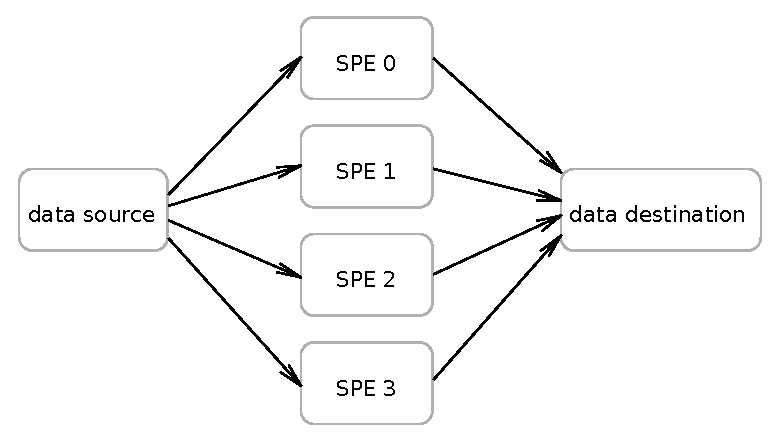
\includegraphics[width=0.9\textwidth]{data/streamingModel}
    \caption[Streaming SPE configuration]{All SPE run the same code creating farm of processor that process same type of data.}
    \label{fg:streamingModel}
\end{figure}

\item Pipeline configuration
\par
SPE server as stages of a pipeline (see figure \ref{fg:pipelineModel}).
Data are passed through from one to other of the SPEs.
The SPE to SPE transfer are faster than SPE to PPE so this can be benefit.

\begin{figure}
    \centering
    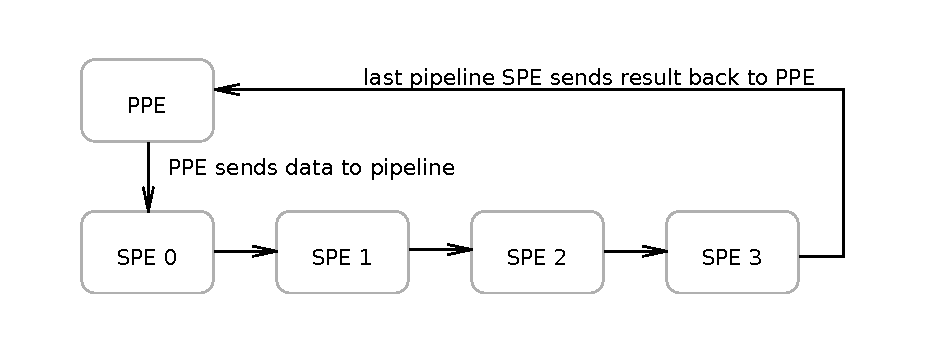
\includegraphics[width=0.9\textwidth]{data/pipelineModel}
    \caption[Pipeline SPE configuration]{SPE creates a pipeline. Each SPE represent one stage of that pipeline. Data are transferred only via SPE to SPE DMA transfers benefiting the speed of bus.}
    \label{fg:pipelineModel}
\end{figure}

\item PPE centric
\par
This configuration is common approach with the Cell/B.E.
Program runs on PPE (see figure \ref{fg:PPUCentricModel}) and only selected, highly demanding computational kernels (hotspots) are offloaded to SPEs.
This method is the easiest from a program development perspective because it limits the scope of source code changes and does not require much re-engineering at the application logic level.
One disadvantage is dynamic changes of SPE contexts that is quite expensive operation.

\begin{figure}
    \centering
    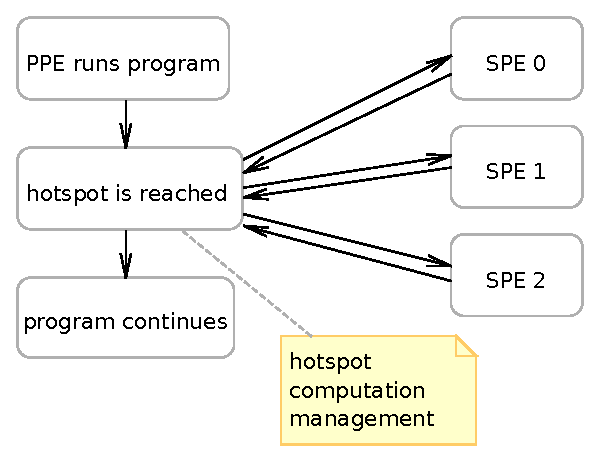
\includegraphics[width=0.7\textwidth]{data/PPUCentricModel}
    \caption[PPE centric configuration]{Program is run on PPE and only hotspots are offloaded to SPEs.
 Offloading means managing SPE context creation and loading as well as managing data transfer and synchronization between PPE and SPEs}
    \label{fg:PPUCentricModel}
\end{figure}

\item SPE server
\par
Another configuration is to have server-like programs running on SPEs that sits and waits offering specific services.
This is requires the code to be small enough to fit into the SPU local store along with processed data.

\end{enumerate}

\section {Building for the Cell/B.E.}
\par
Actual compilation process is performed using appropriate tool chain.
PPE code using of PPE tool chain and SPE code using SPE one.
But there is difference between management of code in linking stage between PPU and SPU object files.
It is caused by difference of actual code usage.
While PPU code resides in central memory, like in common architectures, SPU code is loaded into SPE dynamically and shall be somehow separated.
It is similar to shader programs for graphic accelerators.
They are also loaded into appropriate processors when they are needed so they live separated.

\par
There are two options for SPE code management.
One is to build shared library and load it explicitly when it is used.
Another way is to build a static library and include it into PPU executable using Cell/B.E. Embedded SPE Object Format (CESOF).
This allows PPE executable objects to contain SPE executable i.e. SPE binary is contained within PPE binary.
See figure \ref{fg:SPEEmbedding} how is SPE binary included into PPE binary.
This inclusion is called embedding and is performed with extra tool from tool chain.
The SPU program is then referenced as special external structure direct from PPU code, instead of performing shared libraries loading.
Both ways have advantages and disadvantages which are the same as shared vs. static library usage ones on other platforms.
Shared library means better modularity and possibility of code alternation without whole executable rebuilding.
On the other hand additional management of such library is necessary in contrast to static SPE code into PPE binary embedding.


\begin{figure}
    \centering
    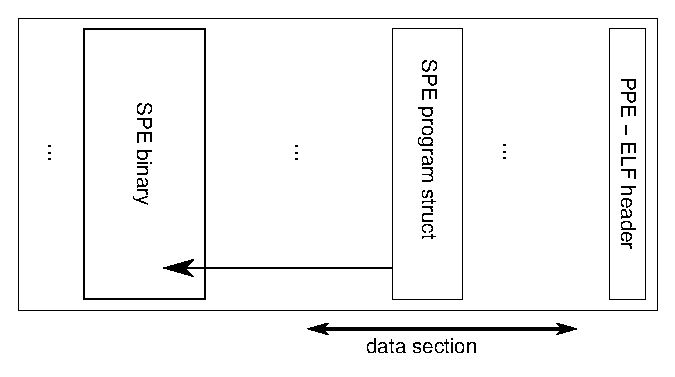
\includegraphics[width=0.8\textwidth]{data/SPEEmbedding}
    \caption[SPE binary embedding]{Illustration how is SPE binary "embedded" into a PPE binary.
An SPE binary is another section of the PPE binary.
It is reachable through extern struct variable, that contains a pointer to the SPE binary.}
    \label{fg:SPEEmbedding}
\end{figure}



\subsection {Process of application porting for the Cell/B.E.}
\label{sect:portingProcess}

Common process of porting an application for the Cell/B.E. processor (figure \ref{fg:appPorting}) consists of next few steps:
\begin{enumerate}
\item Hotspot localization
\par
Through profiling of the application on PPE we find most compute intensive parts, hotspots.
How to profile the application see chapter 5 of \cite{programmersGuide}.

\item Hotspots porting for SPE
\par
Hotspot code is then moved to the SPEs i.e. the code adaptation for SPE features shall be performed.
This means DMA transfers instead of direct memory access, appropriate data structures or other changes utilization.
Data movement tuning, e.g. using different data structures, can be then performed until satisfactory performance is obtained.
\end{enumerate}

\par
Following steps are necessary for application optimization and speed-up.
Application of these steps leads to utilization of all the SPU features such as whole register set utilization, dual-issuing of instructions, SIMD execution and DMA transfers.
More detail in \cite{writingPerfApps} part 4:
\\
\begin{enumerate}
\item{Multi-buffering}
\par
Data that resides within central memory and are processed by SPE should be copied onto local store buffer before actual computation.
When there are more of these buffers the program can take advantage from asynchronous DMA transfer and can process current buffer while the next data are transferred to another buffer.
Then the buffers are simply swapped and the SPU need not to wait until the transfer of next data is complete.
See figure in the paragraph named "Hiding data-access latencies" in \cite{compilerOptions} for illustration.

\item{Branch elimination}
\par
Branchless instruction chain is succession of instructions without any conditional jump.
In other words there is no decision where to continue performed within such succession.
Elimination of branches elongates branchless instruction chain.
In such a chain all data always go through the same instructions that makes possible to perform SIMDation.
There is variety branch elimination methods.
Good information resource provides \cite{cellPerformance}.
This step brings more advantage because branching is problem for every processor.
Branch elimination is probabbly the most complicated step of the porting process.

\item{SIMDation}
\par
Means rewriting scalar code into vectorized to be able to use SIMD instruction.
In this step the most performance gain could be achieved because of multiple data processing by one instruction.
Every single piece of data should go through the exactly same order of instructions in SIMDized code.
Therefore is necessary to have long branchless instruction chain.
The most important method is arrays of structure to structure of arrays conversion.
The figure in the paragraph called "SIMDizing" in \cite{compilerOptions} shall illustrate processing data with SIMD instruction.

\par
SIMDizing brings also avoidance of usage rotation instructions which are necessary to move unaligned data into preferred slot.
Preferred slot is beginning of a register e.g. for short int it is the first 16 bits.

\item{Loop unrolling}
\par
Loop body is the code inside curly brackets of the loop.
This code is executed repeatedly until the loop condition is valid.
Loop unrolling means putting more loop bodies serially into code.
This decrease loop count and elongate the loop body letting the compiler to make more optimizations.
Example:
\begin{verbatim}
for(uint32 i=0; i<32; i++)
{
    printf(".");
}
\end{verbatim}
become (by loop unrolling with factor 2)
\begin{verbatim}
for(uint32 i=0; i<16; i++)
{
    printf(".");
    printf(".");
}
\end{verbatim}
The compiler can do more optimizations e.g. better instruction scheduling and register utilization.

\item{Instruction scheduling}
\par
Proper reorganization of instructions can give us more performance in some cases.
This step is performed by the compiler but it is possible to rearrange instructions manually in assembly language.

\item{Branch hinting}
\par
Give the processor hint where the program is rather going to continue after future branch.
It is done through insertion of special instructions.
This step should be again accomplished by the compiler but is possible to use apropriate assembly language instruction directly within the code.
\end{enumerate}

\par
The whole process is repeated for every single hotspot.

\begin{figure}
    \centering
    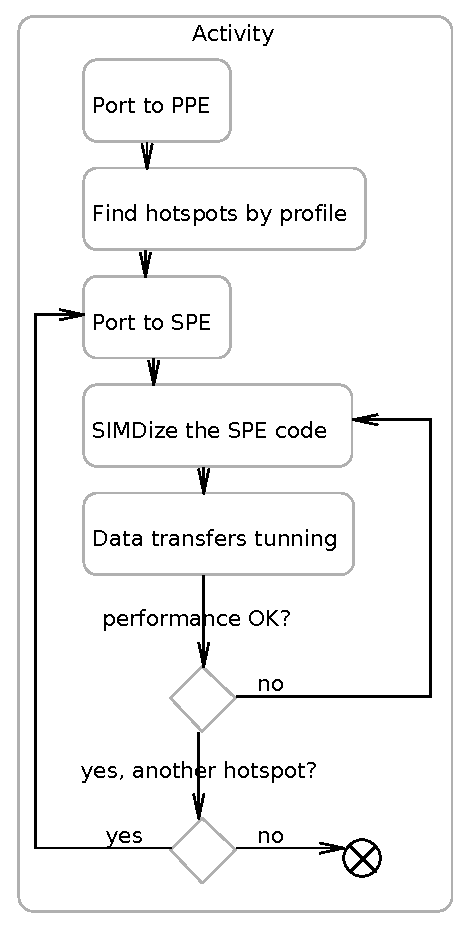
\includegraphics[width=0.5\textwidth]{data/portingCycle}
    \caption[Application porting cycle]{Diagram shows all stages of the process and loops for better performance tuning and other hotspots}
    \label{fg:appPorting}
\end{figure}

\subsection {SPE porting considerations}

\par
Local store size is the main SPE feature that everything spins around while porting code to SPE.
On the one hand are decisions about data transfers.
This means how the data that has to be processed by the SPE will be transferred into local store and vice versa.
What will be the sizes of data chunks.
How many buffers will be used in case of multi-buffering.
On the other hand is code complexity of the solved problem that influence the size of final binary.
There is one solution how to use bigger binaries than the local store, SPE overlays.
It is based on division of the binary into segments that are loaded into SPE on demand in run-time.

\par
Programmer has to take into consideration all these things to make the final binary smaller than local store.
Everything is big tradeoff between processed data chunk sizes with number of buffers of that chunks and code complexity i.e. how large algorithm can be.

\par
When compiling the SPU binary from ported code the final executable will probably increase the local store size even when the code seems not as large as the final binary size.
Then begins big searching what causes this huge size.
We have gone through several problems with code that is common in non SPE code but cause problems in SPE code.
Here is the list:
\begin{enumerate}
\item usage of keyword new
\par
There is no memory allocation on SPE. So new is meaningless.
But compiler accepts it without any complain.

\item usage of std streams
\par
This code:
\begin{verbatim}
#include <iostream>
std::cout << "Hello" << std::endl;
\end{verbatim}
goes through the compiler without complaints but makes the final binary too big.
The reason why the resulting code is too big is probably size of the code within headers that are included when using described features.

\end{enumerate}

\subsection {Speed and compiler options}

\par
There is variety of compiler options.
Usage of them is worth nothing but can increase performance and avoid some kind of bugs.

\par
Mike Acton explains in \cite{strictAliasing} the strict aliasing.
One advantage of usage of this option is its positive impact on performance.
Another advantage is fact that it can avoid bugs that would appear as far as in release stage when optimizations flags are used in compilation.
In this stage is this kind of bugs really hard to track and debug.

\par
Another option advises are in \cite{compilerOptions}

\section{Profiling}

\par
Profiling of Cell/B.E. application means rather profiling SPE part of the application.
There is variety of profiling tools.
The basic one is dynamic performance analysis which can provide many of useful information such as how much time the SPE stall and what reason, the CPI (cycle per instruction) ratio, branch count, etc.
The next one is static performance analysis which can illustrate run of SPE in instruction precision.
These two analysis are evaluated from program run within full system simulator.
Both the methods are well described in tutorial in the cell IDE help which is accessible through menu $\rightarrow$ Help $\rightarrow$ Help Content in IDE.

\par
Another profiling tools are:
\begin{enumerate}
\item{PDT - performance debugging tool}
\item{OProfile}
\item{CPC - cell performance counter}
\end{enumerate}

These tools collect profiling data that can be further processed with VPA (visual performance analyzer), external tool provided by IBM.
This tool can display the collected data in different charts, time lines or can highlight parts of code that are worth to improve and many other useful features.
Usage of all these performance tools is described in SDK document "Performance Tools Reference" in \cite{performanceToolRef}.
We wanted to test them all but when we follow the manual we experienced obstacles because we worked on PS3.
Lately, we found out on forums that unfortunately there is poor or none support for these performance tools on PS3.

\section{Segmentation}


\section{Level set algorithms}

formulace
urychlujici metody
segmentace pomoci levelsetu

\chapter{Design and implementation}

This chapter will describe details of implementation and design of our test application.
It will start with listing of used frameworks continuing with description of the process of the test application incorporation into the frameworks.
After that results of profiling of the application are summarized.
Followed by new design description which was necessary due to unexpected profiling results.
The rest of chapter will present actual porting process with all its problems, solutions, recommendations and all the usable information that we discovered in the porting process.

\section{Original idea of the porting process}

We wanted to follow the common scenario of porting process as described in \ref{sect:portingProcess}.
In our case this means:
\begin{enumerate}
\item{choose base implementation}
\item{clean it up}
\item{port it to PPE}
\item{profile it to find hotspots}
\item{offload hotspots to SPEs and right away to use multi-buffering technique for DMA transfers}
\item{optionally try some optimization steps if the results were not satisfactory}
\end{enumerate}

\section{Chosen algorithm and frameworks}

\par
We decided to choose sparse field algorithm of level set solving for porting to \mbox{Cell/B.E.}
It is a quite complex image processing algorithm that could test the \mbox{Cell/B.E.} programming as a whole.

\par
We took ITK \cite{itk} implementation of that algorithm as a base and have to get familiar with this huge project.
It contains many algorithm implementations as well as necessary infrastructure content such as loading and saving variety of formats.
Base concept of this project is a pipeline and filters.

\par
To get some work done pipeline has to be build from filters.
Filter is an entity that represents an algorithm.
When a pipeline is created the last filter is started.
Starting event then propagates towards the beginning of the pipeline where actual computation starts.
Output from one filter is input of the following one.
Filters thus create a building blocks for some more complicated method.

\par
After several first test with examples and tutorials we wrote our own testing application (originally with code name 'pok').
It was able load image, run the level set filter and save the results.
Some reasonable parameter values were found with the pok application.
It was controlled via bash scripts that is not much easy nor user friendly.
There was also no way how to visualize the results.
So we decided to use another framework to overcome these problems, the MedV4D project \cite{medved}.

\par
This project that was originally started as software project and is basically framework for creation of medical applications.
Its purpose is to simplify process of GUI creation as well as actual computation model design.
Instead the programmer should focus on actual problem solution.
Basic building block is also a filter.
The filter can be merged into pipeline just like in ITK.
But the MedV4D filters are more low-level and thus faster than ITK ones.
The pipeline then offer some implicit locking of data set parts to allow parallel computation.

\section{Incorporation into MedV4D framework}

\par
The most convenient way how to use an ITK pipeline that can be run on the \mbox{Cell/B.E.} seemed the client/server architecture.
So the part of the application that has to be run on the \mbox{Cell/B.E.} is a server.
While client part loads initial data or saves the results, visualize the results and act as GUI with controls for parameter setting.

\par
Whole process can be described as following: a client loads the input data sends them to a server and waits for results.
As soon as the results are read they are visualized.
Then the result can be saved or sent to the server again for computation with another parameters.
See the figure \ref{fg:computationProcess} showing how the application with code name 'LevelSetClient' works.

\begin{figure}
    \centering
    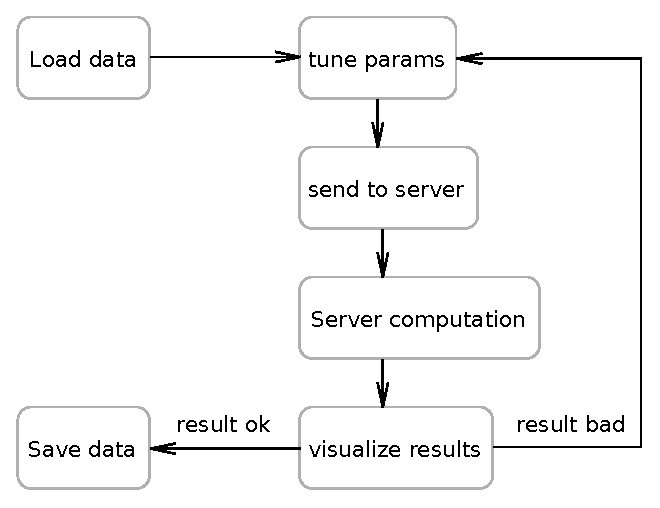
\includegraphics[width=0.7\textwidth]{data/computationProcess}
    \caption[LevelSetClient application computation process]{Client acts like GUI for the server side that performs actual computation}
    \label{fg:computationProcess}
\end{figure}

\par
There were two main goals which were necessary for incorporation pok application into MedV4D framework:
\begin{enumerate}

  \item{Remote computing infrastructure}
  \par
  Infrastructure for sending commands to server along with data or parameter values as well receiving response messages along with resulting data had to be implemented into the MedV4D.
It lead into designing whole new library of the MedV4D called remote computing (RC).
On the client side there is a remote filter that encapsulates whole infrastructure necessary for sending of a pipeline to the server as well as result handling.
The server side had to be designed completely as a whole.

  \item{ITK integration}
  \par
  This is performed by wrapper MedV4D filter that is connected into MedV4D pipeline.
Within this filter there are two ITK images that serves as input and output for inner ITK pipeline.
Actual data of this ITK images point to data of containing MedV4D wrapper filter (see figure \ref{fg:ITKWrapping} for details).

\end{enumerate}

\begin{figure}
    \centering
    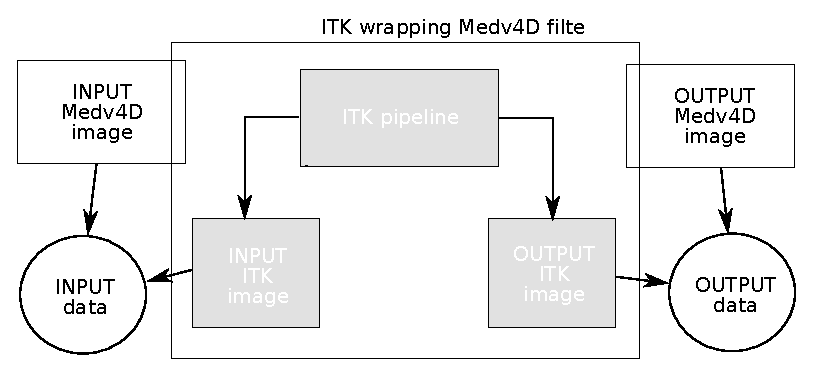
\includegraphics[width=0.9\textwidth]{data/ITKFilter}
    \caption[ITK wrapper MedV4D filter]{Basic elements are the two ITK images whose data are actually MedV4D images' data}
    \label{fg:ITKWrapping}
\end{figure}

\subsection{Client part}

As mentioned above the base element of client RC part is a remote filter.
It implements actual command sending and result receiving functionality.
It is derived from a pipeline MedV4D filter so it can be added into a pipeline.
This part of pipeline that the remote filter represents thus run on a remote server.
Listing of commands that the remote filter issue to the server follows:
\begin{enumerate}
  \item{CREATE}
  \par
  This command is a create request.
It identify the type of the filter that the remote filter represents and that should be instantiated on the server.
Server parses the command message and instantiate appropriate filter along with the whole pipeline (remote pipeline).

  \item{DATASET}
  \par
  Tells the server to read actual data set that the computation will be performed on.
The data set is parameter of the command.

  \item{EXEC}
\par
  This command requests actual execution of the remote pipeline.
But filter parameter values should be parsed before the actual execution.
These values are within the only parameter of this command.
After the parsing and association of filter parameters with the actual filter the remote pipeline is executed.
\end{enumerate}

\par
Purpose of the commands is to divide actual execution into stages and thus to define a state of remote execution.
This is because it would be worthless to send actual data set to server again when user wants to execute the remote pipeline again only with different parameters.
Commands allow this because remote pipeline has state telling 'data already received now waiting for EXEC command as many times as wanted without no more input data transmission'.
\par
The MedV4D pipeline filter defines also some stages that the behaviour of remote filter benefits.
One of them is a method that is called only when input data changes (\mbox{\emph{PrepareOutputDataset}}).
This is perfect place to send DATASET command to server.
Because this is called only on input data change thus DATASET command will be issued on input data change as well.
But CREATE command has to be sent before the DATASET command to build the remote pipeline before data set is transmitted.
CREATE command is sent with DATASET one because remote pipeline has to be recreated every time a new dataset arrives.
\par
And the EXEC command is then send within function that is called when pipeline is executed and that should perform actual computation (\mbox{\emph{ProcessImage}}).
Whole cycle shows the figure \ref{fg:RCClientCycle}.

\begin{figure}
    \centering
    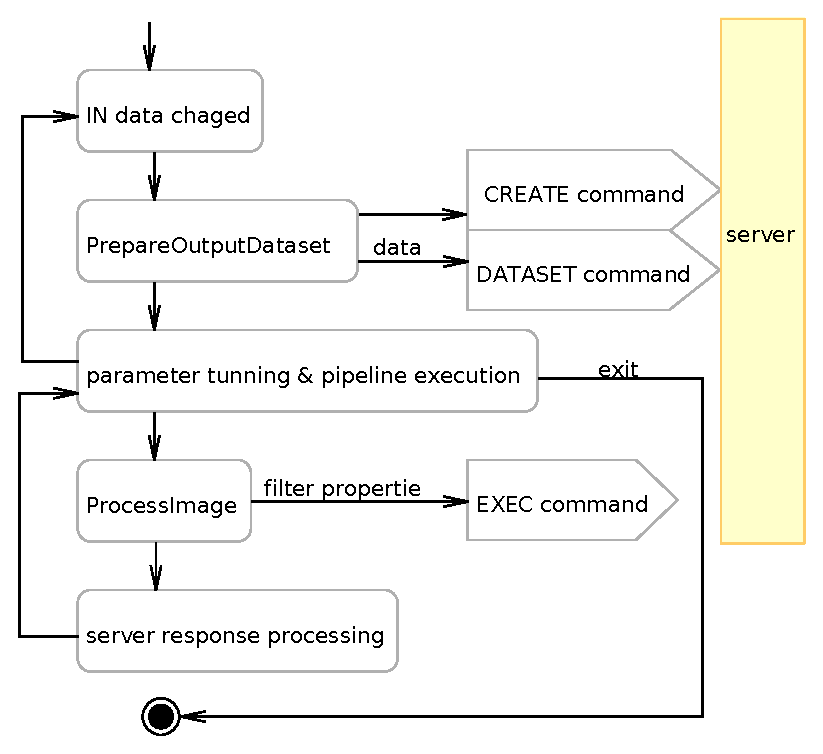
\includegraphics[width=0.8\textwidth]{data/RCClientCycle}
    \caption[Remote MedV4D filter]{Shows three basic states of remote filter and when particular command are sent to server.}
    \label{fg:RCClientCycle}
\end{figure}

Server response can be either OK or FAILED.
In case of OK resulting data set is received in contrast to FAILED case when no data set is expected.

\subsection{Server part}

Server part is counter part of client one so the design reflects it.
Goal of server is to sit and wait for incoming connection.
One connection means one session of computation.
Currently only one session at a time is held.
In context of a session command from client are parsed and appropriate actions performed (see figure \ref{fg:RCServerCycle}).

\begin{figure}
    \centering
    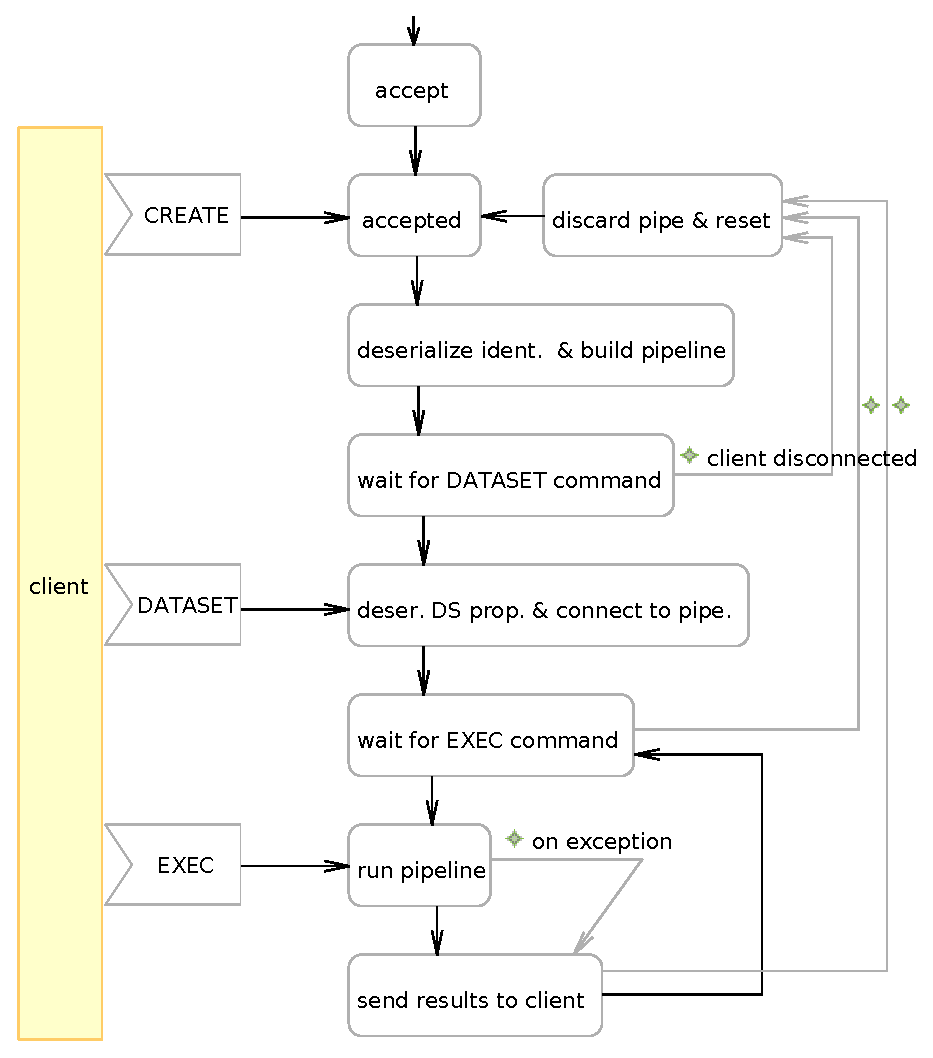
\includegraphics[width=0.9\textwidth]{data/RCServerCycle}
    \caption[MedV4D server cycle]
{
Illustration of server state diagram.
The states correspond to commands that are accepted by the server.
}
    \label{fg:RCServerCycle}
\end{figure}

Like in every client/server application some kind of stubs are needed.
In context of RemoteCellLevelSet application client/server pair the meaning of the stubs are serialization and de-serialization methods.
Goal of the methods is to ensure that data that the client sends will be received in exactly the same order and data types.

\par
Good example is the CREATE request.
In this request identifier of remote filter are sent along with template parameters identifiers (because filter classes are templated).
In case of mismatch of that identifiers completely different class would be instantiated.
Hierarchy of virtual methods on data set classes defines interface for such stubs.
Interface on remote filter properties class hierarchy does the same for the remote filter.

\par
Another issue is endianess.
Endianess identifier is sent along with every command. On the other side is made decision if byte swapping should be performed.
This allows to perform byte swapping only when it is really needed.

\par
Currently only remote filter is implemented - the level set segmentation.
But other filters can be easily added by appending one switch branch in remoteFilterFactory.cpp source.
The level set segmentation filter is implemented as successor of ITK filter that contains appropriate ITK pipeline within.
This pipeline is most interesting part related to this work so further content will be about it.

\section{Level set segmentation pipeline}

This pipeline contains three ITK filters.
\begin{enumerate}
  \item{fast marching filter}
  \par
  Is responsible for initial level set computation.
Parameters of this filter are point $\vec{x}$ in data set and distance $d$.
Output is data set of distances from ball shaped object in the $\vec{x}$ with radius $d$.
This data set is the initial level set front.

  \item{level set segmentation filter}
  \par
  Performs actual level set segmentation method.
Parameters of this filter are threshold interval (thresholding level set segmentation), maximal count of algorithm iterations, curvature and speed scaling (explained above).

  \item{binary thresholding filter}
  \par
  Purpose of this filter is extract resulting object from level set.
It is thresholding that select pixels with values less that zero that corresponds to inner part of the resulting level set.
\end{enumerate}

The fast marching and binary thresholding filter have not been changed and are used as is, part of ITK framework.
The only filter that has been changed was the level set segmentation (LS) filter.
This filter performs the algorithm we have chosen to port to \mbox{Cell/B.E.}, sparse field level set solving.
This algorithm uses linked lists to represent the sparse field layers.
The actual algorithm, as described higher (\ref{alg:sparseFileld}), is implemented in several classes.
These classes form the original LS hierarchy (OLSH).

\section{Pre-porting steps}
\par
Due to the mapping of the algorithm to \mbox{Cell/B.E.} and due to poor lucidity and high universality of ITK code radical changes was necessary.
We decided to rebuild appropriate part of OLSH responsible for the sparse field level set computation.
Our own LS image segmentation filter should be the result of that changes.

\par
There are actually two class hierarchies in the OLSH.
One represents the filter that performs level set algorithm, filter hierarchy.
And the other computes the FDE using the upwind scheme \cite{sethianLS}, finite \emph{difference function} hierarchy.

\par
At the top of the function hierarchy there is \mbox{\emph{FiniteDifferenceFunction}} that computes the upwind scheme with assistance of virtual methods that are implemented in successors.
Successors are:
\begin{enumerate}
  \item{LevelSetFunction}
  \par
  that provides curvature term computation methods.

\item{SegmentationLevelSetFunction}
\par
provides speed image computation infrastructure

\item{ThresholdSegmentationLevelSetFunction}
\par
computes actual speed image
\end{enumerate}

\par
The base of the filter hierarchy is \mbox{\emph{FiniteDifferenceImageFilter}}.
It computes the main loop of level set calculation (see step 1 in \ref{alg:sparseFileld}).
Virtual methods of its successors are used to implement the appropriate sub steps.

\par
The first successor is the \mbox{\emph{SparseFieldLevelSetImageFilter}} providing implementation of algorithm's Step 1a through \emph{update calculation} function.
Other steps are performed by \emph{apply update} function.
Next successors, \mbox{\emph{SegmentationLevelSetImageFilter}} and \mbox{\emph{ThresholdSegmentationLevelSetImageFilter}} only manage \emph{difference function} in appropriate manner.
In case of \mbox{\emph{ThresholdSegmentationLevelSetImageFilter}} this means speed function calculation as described in \ref{eq:speedFunction}.
The function is computed at the beginning for the whole data set into preallocated image.
This image is another notable amount of memory that cannot be accepted for our purpose (see \ref{ps3MemoryUsage}).

\par
Our approach calculates the speed function every time it is needed without any pre-calculations.
This approach could be even better for the \mbox{Cell/B.E.} streaming nature.

\begin{figure}
    \centering
    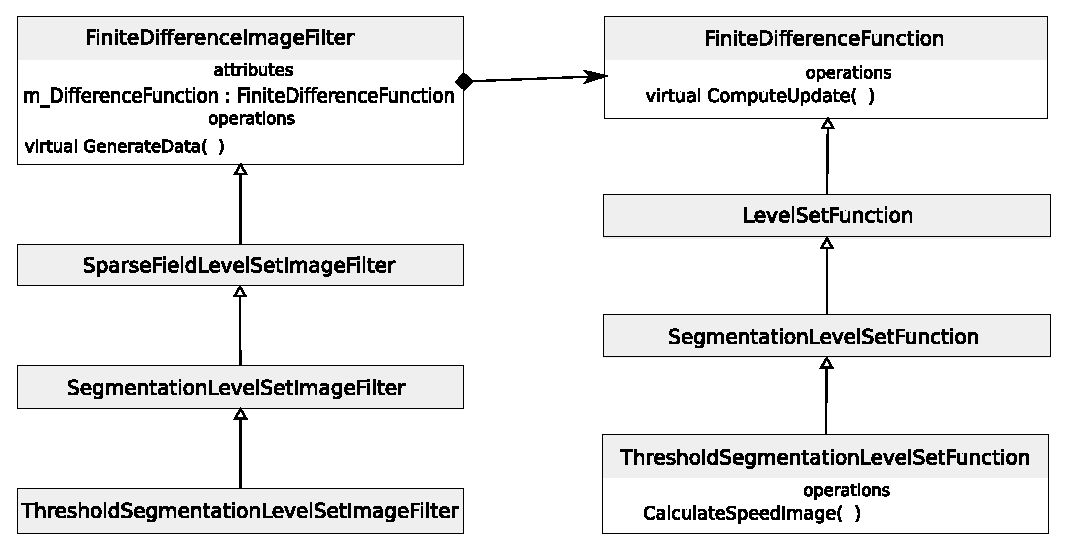
\includegraphics[width=0.95\textwidth]{data/originalHierarchy}
    \caption[Original ITK thresholding level set filter class hierarchy]
{Illustrates the original ITK \mbox{\emph{FiniteDifferenceFunction}} hierarchy and the \mbox{\emph{FiniteDifferenceImageFilter}} hierarchy and their relationship}
    \label{fg:originalHierarchy}
\end{figure}

\par
We have simplified these two hierarchies.
One reason of the simplification was the removal of the pre-calculated image and the other was code clean-up and refactorization.
Result of these changes is our own filter (\mbox{\emph{ThreshSegLevelSetFilter}}, OOF).
It omits all unnecessary part of original LS hierarchy, uses reasonable parts of the original ITK level set segmentation filter (see the figure \ref{fg:resultingFilter}).
It is also ready to be ported for the \mbox{Cell/B.E.}

\par
In the function hierarchy only the base class that the resulting \mbox{\emph{ThresholdLevelSetFunc}} class is derived has left.
This new class does the same job as original LS function hierarchy and omitts the pre-allocation of the speed image.
The computation of particular up-wind scheme terms was separated into standalone classes for more code readability and modularity.
\par
The filter hierarchy was shorted and begins already in \mbox{\emph{SparseFieldLevelSetImageFilter}}.
All its successors in the original hierarchy was omitted since they did anything reasonable for our purpose.
Some function implementation from the \mbox{\emph{SparseFieldLevelSetImageFilter}} was borrowed into the new OOF to be ported for the \mbox{Cell/B.E.}

\begin{figure}
    \centering
    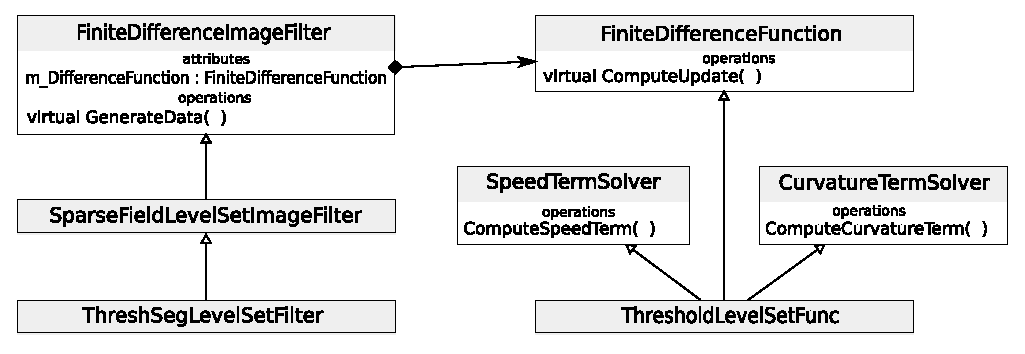
\includegraphics[width=0.95\textwidth]{data/resultingFilter}
    \caption[Resulting level set filter ready to be ported to \mbox{Cell/B.E.}]
    {
Show result of original LS hierarchy rebuilding.
Some unnecessary parts was omitted to clean-up the code and to change behaviour towards streaming architecture as well as term computation was separated into supporting classes for modularity
    }
    \label{fg:resultingFilter}
\end{figure}

\section{Profiling}

As the first step of the porting process the server application with the OOF within was build and profiled with following results:

\begin{table}
\centering
\begin{tabular}{|c|c|c|c|}
\hline
\multicolumn{4}{|c|}{Profiling results}\\
\hline
function name&subroutine&time spend&percent\\&&in calculations&\%\\&&(in seconds)&\\
\hline
\hline
ApplyUpdate()	&				&	20.15&	75.21\\
\hline
		&PropagateAllLayerValues()	&	16.64&	62.11\\
\hline
		&UpdateActiveLayerValues()	&	2.27&	8.47\\
\hline
CalculateChange()&				&	6.11&	22.8\\
\hline
		&ComputeUpdate()		&	3.97&	14.82\\
\hline
TOTAL		&				&	26.79&	100\\
\hline
\end{tabular}
\par
\caption[Profiling results]
{
  Results of profiling showed that \emph{ComputeUpdate} step that was originally thought to be hotspot takes only 14.82\% of computation time.
}
\label{tab:profilingresults}
\end{table}

\par
The profiling (see Table \ref{tab:profilingresults}) shows that the most time consuming parts of the program is not the difference solving in update calculation step but the update application step.
The original idea was to offload only the difference solving within the update calculation step which is performed on $3^3$ voxel matrix and calculated independently of the others which makes this job perfectly suited for offloading to SPE.
But the time taken for computation of this part is only the fragment of the whole.
This is the reason for another changes to OOF.

\section{New design}

\par
Actually the whole OOF had to be rebuild and from original ITK class hierarchy last nothing.
Everything replaced by the OOF and our own version of original \mbox{\emph{FinititeDifferenceImageFilter}} (FDIF) where the main loop of the algorithm as well as stopping conditions resides.
The reason of replacing even the FDIF is that it suppose usage of a difference function and its virtual methods.
But in the new design the difference function will be offloaded as well so it was taken out completely through the our FDIF.

\begin{figure}
    \centering
    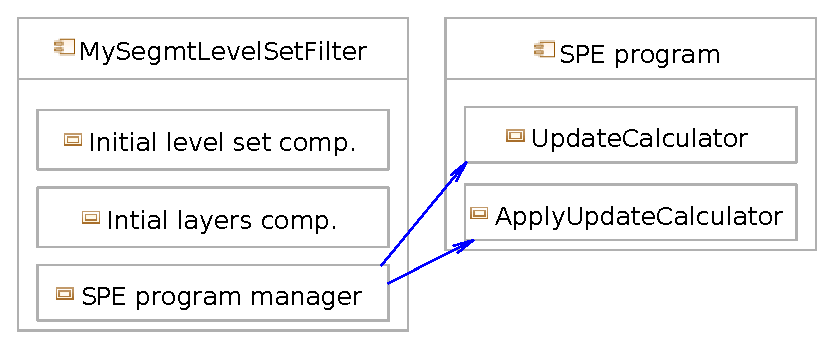
\includegraphics[width=0.9\textwidth]{data/newDesign}
    \caption[Diagram of new design components]
{
Diagram of new design components. Calculation only the initial states is performed by PPE.
And the rest is moved to SPEs through SPEManager that perform all necessary steps to run the SPEs.
}
\label{fg:newDesign}
\end{figure}

In the figure \ref{fg:newDesign} can be noticed that almost whole original ITK pipeline is offloaded to SPE.
Only initialization routines are left to the PPE.
This lead to create the SPE program manager that will manage computations on SPEs.
It is responsible for SPE thread initialization and run, and SPEs synchronization.

SPE part consists of two main parts.
\mbox{\emph{UpdateCalculator}}, performing \emph{update calculation} and \mbox{\emph{ApplyUpdateCalculator}}, performing \emph{update application}.
The \mbox{\emph{UpdateCalculator}} traverse over \emph{layer0} and computes update values for its points.
The computed values are stored in \emph{update buffer}.
It performs STEP 1 of sparse fields algorithm \ref{alg:sparseFileld}.
Then is the \mbox{\emph{ApplyUpdateCalculator}}'s turn that performs the rest of that algorithm on the calculated update values within the \emph{update buffer}.
In context of our implementation the particular steps mean:\\

\begin{itemize}
\item STEP 2
\par
For every \emph{layer0} compute new level set value and perform test if it stays in the interval [-$\frac{1}{2}$,$\frac{1}{2}$].
If not, move the point into appropriate status list.
This is performed by \mbox{\emph{UpdateActiveLayerValues}} method.

\item STEP 3
\par
Is performed by sub-component of \mbox{\emph{ApplyUpdateCalculator}}, the \mbox{\emph{LayerValuesPropagator}}.
This traverses over all layers, process their values and remove nodes eventually if they are no longer in a layer.
Step processed by \mbox{\emph{PropagateAllLayerValues}}.

\item STEP 4
\par
Traverse over status lists in innermost to outermost order and process their nodes.
If needed a node is moved to inward (outward) status list and simultaneously appropriate layer.
This is performed by \mbox{\emph{ProcessStatusLists}} method.
\end{itemize}

\subsection{Data flow}

\par
In porting process is necessary to know the data flow i.e. find out what data are sent and where.
What data are there produced and especially the size of all the data.
This is because of decision where they will be stored.
Whether in SPE local store or in central memory.
For the first case their size has to be limited because of limitation of local store.
For the second case communication via DMA will be necessary but the data size is not limited to small local store.

\par
There are both cases in our application.
\mbox{\emph{ProcessStatusLists}} method can be performed completely within an SPE without loading any data from central memory.
But the rest of processed data is too big and can not reside within the SPE and has to be DMAed in chunks from central memory.
The big data are statuses, actual level set values and features that are stored within status, output and feature images.
So it is necessary to load and store parts of that images for methods described above.
Computation is performed on small neighbourhood of voxels 3x3x3 (neighbourhood).
So 27 voxels (resp. statuses) has to be transferred for one node processing.
Another big data are nodes within actual layers, linked list chains of nodes.
Traversal over such chains is performed sequential by loading one node after another.
For each loaded node one or more neighbourhoods shall be loaded.
The computation is then performed on those neighbourhoods.

\par
There are other data that have to be stored within central memory and that contribute to the data flow as well.
Next list describe what data are processed in most important methods resp. steps within our application:\\

\begin{itemize}
\item UpdateCalculator
\par
Needs an array which is as long as the layer0.
The size of the layer can be very big so it is impossible to store it within SPE local store.
Therefore the array has to reside in central memory and its content has to be load into SPE local store buffer while the list traversal.

\item \emph{UpdateActiveLayerValues}
\par
Process the array from UpdateCalculator so it has to load it from central memory.
It operates on layer0.
Some nodes are moved into status list and simultaneously \emph{UNLINKed} from layer0 list.
Layer resides in central memory so beside the loading nodes for traversing, some special operation has to be defined which perform the \emph{UNLINK} action.
\par
Status lists are temporary objects. They live only during one \mbox{\emph{ApplyUpdateCalculator}} turn.
So they can reside within SPE's local store.
So no special operation communicating with central memory has to be defined.
But processing of the list0 has to be changed.
In original ITK code the \mbox{\emph{UpdateActiveLayerValues}} operates on the whole layer0.
This one call can produce too long status lists that will not fit into local store.
So iteration over layer0 has to be limited to produce limited length status lists.
We have defined the limit with constant \mbox{MAX\_TURN\_LENGHT} and call processing the limited segment of layer0 a 'turn'.
%See figure \ref{fg:updateActiveLayerValues}.

\item \emph{ProcessStatusLists}
\par
Works on the limited length status lists.
During the lists processing some nodes are moved from one to another layer which means they have to be unlinked from one and linked into another.
Linking to another layer defines another layer operation, \emph{PUSH}.
One status list is processed untill empty so all status lists remains empty and thus ready for the next \emph{UpdateActiveLayerValues} turn after \emph{ProcessStatusLists}.

\item \emph{PropagateAllLayerValues}
\par
This method traverse over all the layers and performs moving nodes among the layers.
This means operations \emph{PUSH} and \emph{UNLINK} as well as layer traversal and appropriate neighbourhoods loading.
\end{itemize}

%\begin{figure}	//TODO {data/updateActiveLayerValues}

\par
There are some actions and operations defined above that need communication with central memory.
This is parts of program where cell PPE - SPE communication features take place.
Other SPE code need not to know if it is run on SPE or PPE.
Therefore set of tools that performs PPE - SPE communication was developed.

\subsection{Tools}
Tools are parts of the program that perform data transfer between PPE and SPE.
All these tools perform multi-buffering to avoid waiting for data.

\begin{enumerate}
\item \emph{NeighbourhoodCell}
\par
Represent the part of an image ($3^3$ voxel matrix) needed for one node computation.
It uses transfer list that allow data handling in scatter-gather manner.
Neighbourhoods are grouped within \mbox{\emph{PreloadedNeigborhoods}} container that manages which neighbourhood is being loaded, used in computation or saved i.e. actually performs multi-buffering.

\item \emph{RemoteArrayCell}
\par
Represents an array stored in the main memory.
This tool is used for UpdateCalculator to save computed update values and in \mbox{\emph{ApplyUpdateCalculator}} to retrieve the values which \mbox{\emph{UpdateCalculator}} has stored.
Its role is to perform DMA transfers not along each value save but on a buffer of that values.

\item \emph{LinkedChainIteratorCell}
\par
It traverse over a layer which is linked list data structure.
As soon as one item is retrieved, transfer of the next one is immediately started.
\end{enumerate}

\par
\emph{PUSH} and \emph{UNLINK} operations are related to linked chains of nodes, the layers.
We decided to implement them using mailboxes.
Mailbox is another SPE to PPE communication channel which is able to transfer 32bit integers synchronously.

\par
Because of the 32bit integers transfer limitation actual \emph{PUSH} and \emph{UNLINK} parameters have to be decoded and encoded.

\begin{enumerate}
\item \emph{PUSH}
\par
Has to push a node into specified layer.
Voxel coordinates and number of layer is encoded and sent over mailbox to PPE.
On the other side the PPE creates a new node appropriately and puts it into specified layer.

\item \emph{UNLINK}
\par
Operation has to unlink a node from a specified list.
Address of that node along the layer number are the parameters.
Address is transferred in 32 bit chunks (because mailbox has 32 bit size) which are decoded on the PPE side to actual node address that is then unlinked from specified layer.
\end{enumerate}

\par
Another support tool that is worth mention is \emph{ObjectStore} which is simple memory allocator templated with class of items it provides and size of an array that the items are taken from.
Provides two main methods, \emph{Borrow} and \emph{Return}.
It is used for allocation of status field nodes.
They reside in local store and thus should be allocated on the stack.

\par
Great advantage of the tools is also that the whole code uses only the tools for central memory communication.
Therefore debugging transfer issues means debugging the tools.

\subsection{Work balancing}

\par
The sparse field layers are central part that defines the amount of work to be performed.
So it is necessary to balance their length among the SPE that process them.
This work is left to \emph{Work manager}.
Its goal is to ensure that all the layers are divided among SPE uniformly.

\par
For this purpose the \emph{UNLINK} and \emph{PUSH} operations implemented using mailboxes fits well.
The idea behind is that actual operation on the linked list is delegated to the \emph{Work manager}.
It decides which SPE layer segment should the node appended into.

\par
The whole process can be compared with company department where are several workers doing actual work and one manager who distributes the work among the workers.

\section{Actual porting process}

\par
Here we will describe our experience with actual porting procedure, problems that the procedure has brought and our solutions of those problems.

\subsection{PC as \mbox{Cell/B.E.} simulator}

\par
Because remote debugging program running on PS3 is quite time consuming (seconds step into command and the like) and because of small amount of memory (see paragraph \ref{ps3MemoryUsage}) we decided to left actual porting to the very end of the process.
Features that are needed for running on SPE were gradually added into the original code.
Some parts were rewritten (e.g. the \emph{UpdateActiveLayerValues} turn) to allow some data to live in SPE local store.
All the changes have not changed the programs' output, so one can say that the all the programs in every step are equivalent.
All the debugging was performed on PC platform locally and thus quickly.
The \mbox{Cell/B.E.} special features like DMA transfer was simulated by memcpy or the mailbox issues trough simple queue.

\subsection{Moving to PPE}

\par
It seems that moving the code to PPE is easy and there could be no problem.
But we faced a problem that is worth to mention.
Because our code uses lot of third party libraries there are quite much paths to include folders.
It is necessary to manage them well and not to mix architecture dependent ones.

\par
We have mixed up include files of the boost library when cross-compiling and experienced totally strange behaviour.
We thought that we can use boost library includes that come from repository for i686 architecture.
The code crashed on boost code that should be debugged and stable.
For instance opening a file has crashed for unknown reason.
When program was compiled with includes from ppc(64) repository all problems have disappeared.

\subsection{Tools porting}

\par
Next step was to port the tools for SPE.
In fact is to rewrite usage of memcpy that simulate the DMA transfer to use real DMA transfer.

\par
Data that are transferred through DMA (DMAed) within the \mbox{Cell/B.E.} should meet size and align conditions (see \cite{programmersGuide}, Chapter 4).
Data that does not meet this condition will generate BUS error.
This condition forced that all data that are DMAed should be allocated onto aligned addresses (see objectStore.h or updateValsAllocator.h).

\par
Debugging within this step is performed already on a \mbox{Cell/B.E.} machine.
We used both PS3 and systemsim.
Systemsim can detect which DMA transfer brakes align rules and thus cause the BUS error but it is really slow.
Instead using systemsim we have implemented DMAGate (see DMAGate.h) that all DMA transfer go through and where are all the conditions checked.
Such central point for all DMA transfer is really important part of \mbox{Cell/B.E.} program because it gathers all DMA stuff into one place making debugging much more easier.

\subsection{Memory checking tools}

\par
Gradual code porting for SPE was really time consuming due to fact that tools operates with a stack memory.
Debugging such parts needs extra care for what is where rewritten.
Since we are using a stack memory some part of call stack would become corrupted and program becomes undefined.
The worst thing is that it can continue without crash or to crash on totally different place.
Errors of this type are always hard to track.
There is need of usage of some checking tools.
For us memcheck tool, part of Valgrind, proved to be useful to detect stack corruption.

\par
Usage of DMA transfers (or memcpy) is also dangerous.
It rewrites destination memory without checking what is within that memory.
Then many errors causing segmentation faults arise.

\par
We have spent lots of time debugging many of such errors.
Even in resulting application can occur some errors of this kind.
Debugging every single this kind error is a never ending story.
So we recommend to write additional tools that will check such errors or to use memory checking software such as Valgrind \cite{valgrind}.
We used the Valgrind but not from the beginning.
So when we check the program there was too much warnings of the same kind.
Solving them was in that time impossible.

\par
Checking the program with memory checking tools is necessary already from the very beginning of the development and quite often.
It is advisable not to make huge code changes not only due to memory checking but due to actual process as such.
It is better to develop gradually in small steps.
One can then find error more simply.
This is universal rule for programming but we believe it is valid specially for the \mbox{Cell/B.E.} porting process.


Tabulka:::
\begin{center}
\begin{tabular}{|l|c|p{3.5in}|}
\hline
\multicolumn{3}{|c|}{Nazev tabulky}\\ 
\hline cell 1&cell 2&cell 3\\&todle bude pod cell 2, protoze to je mezi dvema'\&' &\\ 
\hline Big Basin&1.5&Very nice overnight to Berry Creek Falls from
either Headquarters or ocean side.\\ 
\hline Sunol&1&Technicolor green in the spring. Watch out for the cows.\\ 
\hline Henry Coe&1.5&Large wilderness nearby suitable for multi-day treks.\\ 
\hline
\end{tabular} 


%--------------------------------------------------------
%-------------          REFERENCE           -------------
%--------------------------------------------------------

\bibliographystyle{plain}
\bibliography{references}

\appendix
\chapter{Tools setup}
\label{toolsSetup}

\section{SDK installation}

As first you have to do is to download actual SDK.
Go to \url{http://www-128.ibm.com/developerworks/power/cell/ downloads.html?S_TACT=105AGX16&S_CMP=LP}.
You should download following files:

\begin{enumerate}
\item SDK 3.1 Installer
cell-install-3.1.0-0.0.noarch.rpm  (11MB), contains install script and other stuff for SDK installation.
\item SDK 3.1 Developer package ISO image for Fedora 9
CellSDK-Devel-Fedora\_3.1.0.0.0.iso  (434MB), contains rpm packages that actual SDK is composed from (SDK packages)
\item SDK 3.1 Extras package ISO image for Fedora 9
CellSDK-Extras-Fedora\_3.1.0.0.0.iso  (34MB), contains some extra packages for Fedora
\end{enumerate}

Download it wherever you want (even though in documentation is /tmp/cellsdkiso).
Lets call the folder, you download it into, ISODIR.
First you shall stop the YUM updater daemon.

\begin{verbatim}
/etc/init.d/yum-updatesd stop
\end{verbatim}

If this outputs: bash: /etc/init.d/yum-updatesd: No such file or directory, you do not have any YUM updater daemon installed so you can skip this step.
Now issue following command to install required utilities for SDK installation

\begin{verbatim}
yum install rsync sed tcl wget
\end{verbatim}

Now install the downloaded installation rpm.

\begin{verbatim}
rpm -ivh ISODIR/cell-install-3.1.0-0.0.noarch.rpm
\end{verbatim}

After this step you have new stuff in /opt/cell installed. There is SDK installation script (cellsdk) located as well.
It is wrapper for YUM that manages the SDK packages. Run it with parameter --help to see the usage.
So next step is to run it.

\begin{verbatim}
/opt/cell/cellsdk --iso ISODIR -a install
\end{verbatim}

Parameter --iso tells to use downloaded ISOs and where can be found for mounting them onto loop-back device.
Parameter -a disables agreeing licenses. Otherwise you have to write some 'yes' to agree.
Process begins with setting local YUM repositories pointing to the ISOs.
Then all default packages are installed with all their dependencies.
To check result of the installation issue

\begin{verbatim}
/opt/cell/cellsdk verify
\end{verbatim}

Now we have SDK installed. Lets continue with installation of IDE.
It consists again of packages.
Now to simplify processing packages install yumex that provides graphical interface to YUM.
And lets you simply check packages that you want.

\begin{verbatim}
yum install yumex
\end{verbatim}

To install CellIDE run yumex, go to Group View$\rightarrow$Development$\rightarrow$Cell Development Tools.
Check \textit{cellide}, that is actual IDE (Eclipse with cell concerning stuff) and \textit{ibm-java2-i386-jre}, that is Java Runtime Environment, JRE needed for running of IDE.
And click 'Process Queue'. Note: you should have the ISOs mounted onto loop-back devices.
Otherwise you get 'Error Downloading Packages' after clicking 'Process Queue'.
So you have to mount ISOs whenever you want to install package concerning Cell SDK

\begin{verbatim}
/opt/cell/cellsdk --iso ISODIR mount
\end{verbatim}

After the installation you have two new folders.
/opt/cell/ide that contains the IDE and /opt/ibm/java2-i386-50 where JRE resides.
To run the ide you have to specify folder where the JRE is (through -vm param).

\begin{verbatim}
/opt/cell/ide/eclipse/eclipse -vm /opt/ibm/java2-i386-50/jre/bin/
\end{verbatim}

\section{IBM Full-System Simulator}

The last part of development environment is IBM Full-System Simulator (systemsim).
It is not part of ISOs with SDK so you have to download it separately.
Visit \url{http://www.alphaworks.ibm.com/tech/cellsystemsim/download} and download rpm with the simulator appropriate to the platform you are currently using.
Be sure to download fedora 9 version of the simulator (cell-3.1-8.f9.*). Then install it.

\begin{verbatim}
rpm -ivh ISODIR/systemsim-cell-3.1-8.f9.i386.rpm
\end{verbatim}

Maybe some dependencies will be missing. So you have to install it. In my case ot was libBLT24 and libtk8.5.

\begin{verbatim}
yum install blt tk
\end{verbatim}

Now you have simulator installed. But it has nothing to simulate.
Image with image of simulated Fedora 9 system is needed (sysroot image).
It is among SDK rpms so install it using yumex (Cell Development Tools$\rightarrow$sysroot\_image).
Now all necessary stuff is installed.
 You could start the IDE and start development. But there are some bugs to fix yet.

\subsection{Bug fixing}

If you start IDE and it crashes with unhandled exception it is probably caused by xulrunner library.
It is usually installed with Firefox3. There is following workaround:
\begin{enumerate}
\item download an older version of xulrunner

e.g. from: \url{http://releases.mozilla.org/pub/mozilla.org/xulrunner/ releases/1.8.1.3/contrib/linux-i686/ xulrunner-1.8.1.3.en-US.linux-i686-20080128.tar.gz}

\item untar to accessible directory

Lets call it XULDIR

\item edit the file

/opt/cell/ide/eclipse/eclipse.ini file as follows:
\label{XULLFIX}
\begin{verbatim}
...
-vmargs
-Dorg.eclipse.swt.browser.XULRunnerPath=XULDIR
...
\end{verbatim}
\end{enumerate}
Now you should start the IDE without the crash.

\par
Another issue (stack issue) is with tcl (scripting language that is used for configuration of the systemsim).
There is bug with stack size checking that causes cycling of tcl code.
To workaround this problem you should use ulimit command that changes default environment of Linux programs

\begin{verbatim}
ulimit -s unlimited
\end{verbatim}

causes that stack is unlimited.

\par
The last is to fix actual tcl script that manages loading the sysroot\_image (21\% issue - loading of the sysroot\_image freezes on 21\% so is not started and thats why unusable).
It is cause by wrong triggers that are triggerd when some text is output from console by the sysroot\_image loading.
There is probably triggers that wait for text from previous version of SDK that is never output in the current version.
That is why the loading freezes on 21\%.
To fix it you have to edit /opt/cell/ide/eclipse/plugins/ com.ibm.celldt.simulator.profile.default\_3.1.0.200809010950/ simulator\_init.tcl file.
Replace the "Welcome to Fedora Core" string with "Welcome to Fedora" and "INIT: Entering runlevel: 2" with "Starting login process".

It is useful to create starting script. That solve the stack issue and add systemsim directory to PATH (needed for running).

\begin{verbatim}
ulimit -s unlimited
PATH=/opt/ibm/systemsim-cell/bin:\$PATH
/opt/cell/ide/eclipse/eclipse -vm /opt/ibm/java2-i386-50/jre/bin
\end{verbatim}

\subsection{Installation of libraries into sysroot\_image}

Because sysroot\_image is provided as image of installed Fedora 9 without Cell B.E. libraries so next step is to install them into sysroot\_image.

\begin{verbatim}
/opt/cell/cellsdk_sync_simulator install
\end{verbatim}

This shell script installs all rpms for ppc and ppc64 platforms that finds in /tmp/cellsdk/rpms.
By default these rpms are copied into /tmp/cellsdk/rpms during the install process.
If they are not still there (or in installed subdirectory) you have to copy them by hand from ISOs (note: ISOs has to be mounted).

\begin{verbatim}
cp /opt/cell/yum-repos/CellSDK-Devel-Fedora/rpms/*.{ppc,ppc64}.rpm\
/tmp/cellsdk/rpms
\end{verbatim}

\subsection{Copying content into sysroot\_image}

Sysroot\_image is common binary image that can mounted and thus some additional content copied into.
This is useful when extra library that are not part of the default image need to be used.
In my case that was some boost libraries. So to mount the sysroot\_image issue:
\begin{verbatim}
mount -o loop /opt/ibm/systemsim-cell/images/cell/sysroot_disk <your mount point>
\end{verbatim}
And then copy whatever you want.

\subsection{Simulator hints}

\par
You can ssh to running simulator. It is better to use real bash that the console within IDE.
You have all the bash advantages like command and path completion available in contrast to 'text mode' of the IDE console.

\par
Sometimes root user is needed for an operation performed in the simulator.
Its password should be disabled.
It can be done when sysroot\_image is mouned.
Under host machine root account the sysroot\_image\_mount\_point/etc/passwd file should be edited.
The first line is the root's so deletion of '*' characted from the second field (after the second ':' character) will disable the root's password.
Note that this action must be performed when the simulator is not running otherwise the changes will be overwritten by the simulator.

\section{Setup CellIDE}

\section{Using examples}

Examples are installed into /opt/cell/sdk/src as tarball. So you have to untar each you want to use.
It is good to start with examples and tutorial sources.
Each folder has its own makefile that manages makefiles in its sub folders.
 So you can call only the top level one to build all projects in sub folders or any from the sub folders to build particular projects.

It is convenient to use the sample sources in CellIDE where you can build it as well and create run/debug configuration for running within cell environment.
To use the example code (for example /opt/cell/sdk/src/tutorial/simple) create new c++ makefile project.
Click right button on it to get into properties.
C/C++ general tab $\rightarrow$ Paths and Symbols $\rightarrow$ Source location.
Here you have to add the folder with the sources (/opt/cell/sdk/src/tutorial/simple) by 'create / link folder' button $\rightarrow$advanced $\rightarrow$ link to folder in filesystem.
Now you have two folders in list. The first one is the original, created during project creation and the other newly linked folder with the source.
You can delete the original one since you are not going to use it.
Next is necessary to set up 'Build directory' to tell the IDE where shall search for makefile.
It is C/C++ Build tab. Use 'Workspace' button to specify the folder because it will use workspace\_loc variable and thus independent on exact location on filesystem.

\section{Tuning memory usage on PS3}
\label{ps3MemoryUsage}

PS3 has only 256MB RAM memory. This is very small amount for operating system and programs together.
When install fedora system with default state and boot up it, the amount of remaining free memory is about 10MB.
It is insufficient for either debugging and compilation.
So some of resources has to be switched off.
Our PS3s are accessed remotely via ssh so there is no need for X server.
So this is the first you can turn off. This is performed by change of runlevel from 5 to 3.
Run level setting is in /etc/inittab file:
\begin{verbatim}
change in line "id:5:initdefault:" the 5 to 3
\end{verbatim}
Another resource are services.
Here you have to consider if the service you want to turn off is really unnecesary.
In Our PS3 NeworkManger and Wireless supplicant was turn off.
NOTE: when you turn off network manager, you have to turn on network service otherwise the networking will not run properly.
For service management within ssh console /usr/sbin/ntsysv manager is quite useful.
After disabling all unnecessary services we got about 130MB of free space.

Yellow dog distributions goes even beyond. They can access other 256MB in PS3 locked for graphics.
Special device is created and the graphic memory is the used as a swap partition. For details see \url{http://us.fixstars.com/products/ydl/}.

\section{Performance tools}

\begin{verbatim}
yum groupinfo "Cell Performance Tools"
\end{verbatim}

\section{Visual Performance Analyzer - VPA}

Another useful tool is VPA. It is not part of SDK so it should be downloaded separately.
Visit \url{http://www.alphaworks.ibm.com/tech/vpa} for details.
After installing (actually unpacking) the downloaded file similar fix in ini file to eclipse.ini file (see\ref{XULLFIX}) should be done to run the VPA correctly.
\chapter{Content of the DVD}

\par
There is an index.htm that could be used as starting point.
It points to this thesis as well as to install all additional third party content required by test applications.
There are also instructions how to compile and use attached code and data.

\par
The index file also contains user documentations of all the test applications.

\end{document}